\section{斜面}\label{sec:8-4}

在把重的物体搬到车上时,我们常常搭上一块木板,沿着木板把物体推上去(图 \ref{fig:8-6} 甲),这样的木板就是斜面。

斜面也是一种常用的简单机械。在学过功的原理后,我们很容易懂得斜面的原理,知道使用它有什么好处。

我们用图 \ref{fig:8-6} 乙所示的直角三角形 $ABC$ 来研究斜面的作用,其中 $AB$ 是斜面的长用 $l$ 表示,
$BC$ 是斜面的高用 $h$ 表示,$G$ 表示物体重, $F$ 表示沿着斜面推动物体所用的力。

\begin{figure}[htbp]
    \centering
    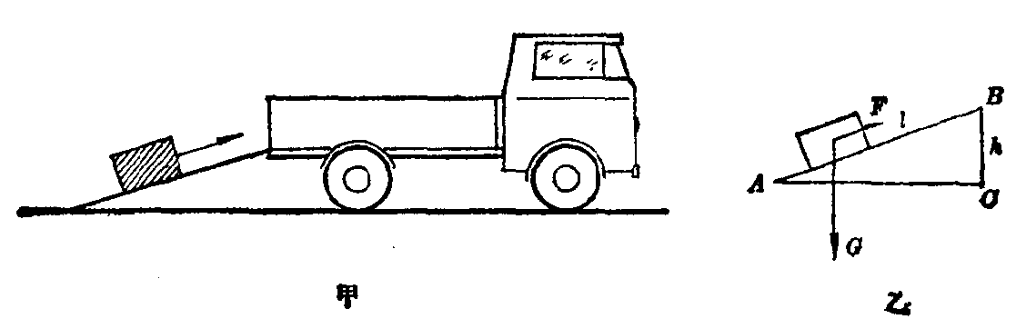
\includegraphics[width=0.8\textwidth]{../pic/czwl1-ch8-6}
    \caption{}\label{fig:8-6}
\end{figure}


从功的原理知道,使用任何机械都不能省功。
所以沿着斜面把物体匀速推上去所做的功 $Fl$,应该等于不用斜面而直接把物体抬上去所做的功 $Gh$,
即 $Fl = Gh$,这个式子可以改写成
$$ \dfrac{F}{G} = \dfrac{h}{l} \;\juhao $$

\textbf{上式表示斜面长是斜面高的几倍,所用的推力就是物体重的几分之一}。
可见,\CJKunderwave{使物体升高相同的高度,斜面越长越省力}。

根据功的原理得出的上述结论,可以用实验来验证。如图 \ref{fig:8-7} 所示。
先用弹簧秤把一个小车匀速地竖直提上去,记下弹簧秤的读数 $F_1$。
然后,用弹簧秤沿斜面把这个小车匀速地拉上去,记下弹簧秤的读数 $F_2$。
换用一个高度相同但是更长的斜面,用弹簧秤沿着这个斜面把小车匀速地拉上去,记下弹簧秤的读数 $F_3$。
从实验结果可以看出 $F_1 > F_2 > F_3$,即利用斜面可以省力,而且在高度相同的情况下,斜面越长越省力。

\begin{figure}[htbp]
    \centering
    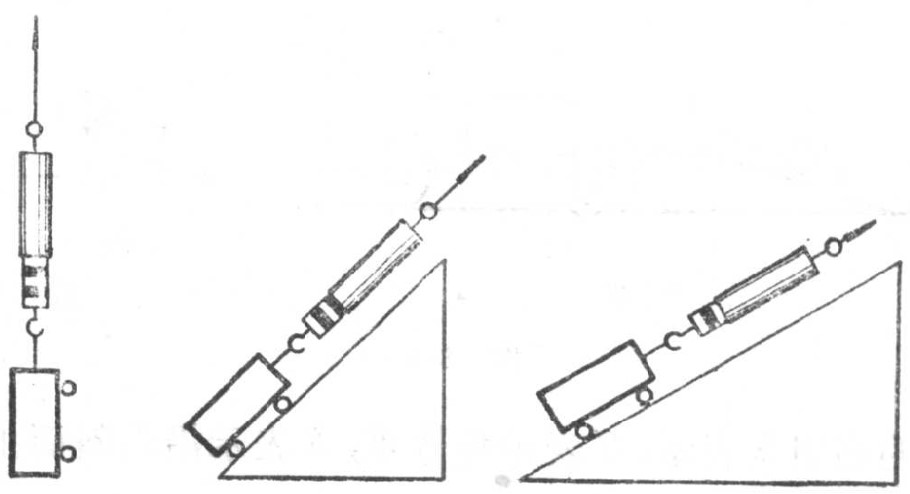
\includegraphics[width=0.6\textwidth]{../pic/czwl1-ch8-7}
    \caption{}\label{fig:8-7}
\end{figure}

\begin{figure}[htbp]
    \centering
    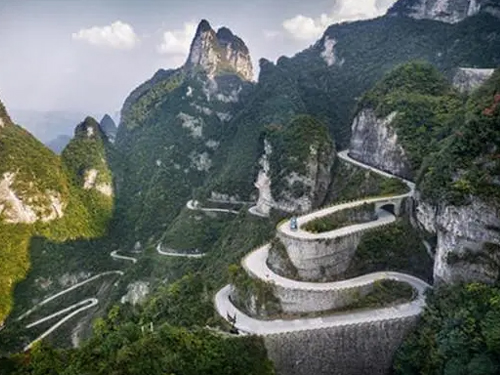
\includegraphics[width=0.5\textwidth]{../pic/czwl1-ch8-8}
    \caption{}\label{fig:8-8}
\end{figure}

利用斜面,我们多通过了距离,但是省了力。
山区的公路修得盘旋曲折(图 \ref{fig:8-8} \footnotemark),延长了爬坡的距离,就是为了省力。
\footnotetext{注:原书的图模糊不清,我从网上找了一张据说是“崇山公路”的图片来替代。}%原书图片保存为 pic 目录下的 czwl1-ch8-8.old.jpg



\lianxi

(1) 同样高的两座山,爬比较陡的那座山比较费力,为什么?

(2) 骑自行车上坡,走 $S$ 形路线比较省力。为什么?

(3) 矿坑里一条坑道长 120 米,坑道两端的高度差是 20 米,
沿着这条坑道拉上一辆 1.2 吨的矿车,要用多大的拉力?摩擦力忽略不计。

(4) 一个山坡每 100 米升高 25 米,用 25 牛顿的力把一个雪撬拉上这个山坡,
这个雪撬有多重?摩擦力忽略不计。


